\documentclass{article}
\usepackage{scribe}
\usepackage{amssymb}
\usepackage{amsmath}
\usepackage{graphicx}
\usepackage{subcaption}
\usepackage{pgfplots}
\usepackage{listings}
\usepackage{float}
\usepackage{wrapfig}
\usepackage{lscape}
\usepackage{listings}
\usepackage[utf8]{inputenc}
\usepackage{leftidx}

\newtheorem{hw}{Homework Problem}
\newtheorem{ex}{Example}

\newcommand{\Perp}{{\bot\negthickspace\negthickspace\bot}}


%%% Unless you have very specific needs, the lines above should include
%%% all the typesetting features you need.

 


\begin{document}
% \begin{lecture}{September 4th, 2004}{Ao Zhang}



\section{Results without regularization}

Since there are $3$ changing parameters ($N$, $d$, and $\sigma$), we will focus on $1$ parameter each time in the following subsections with fixing the other parameters. Other parameters are set as:\\
1. $\mathcal{D}_{test} = 2000$ and $\mathcal{D}_{bias} = 3000$;\\
2. $\alpha_{learning} = 0.1$ with decay $0.96$ after each $100$ steps;\\
3. $epoches = 1000$ for iteratively update loss function.

\subsection{Result of different complexities}

Complexity is researched at first, the result is plotted as Figure~\ref{fig:complex_nonreg} shows,
\begin{figure}[h]
\centering
\begin{subfigure}{.45\textwidth}
  \centering
  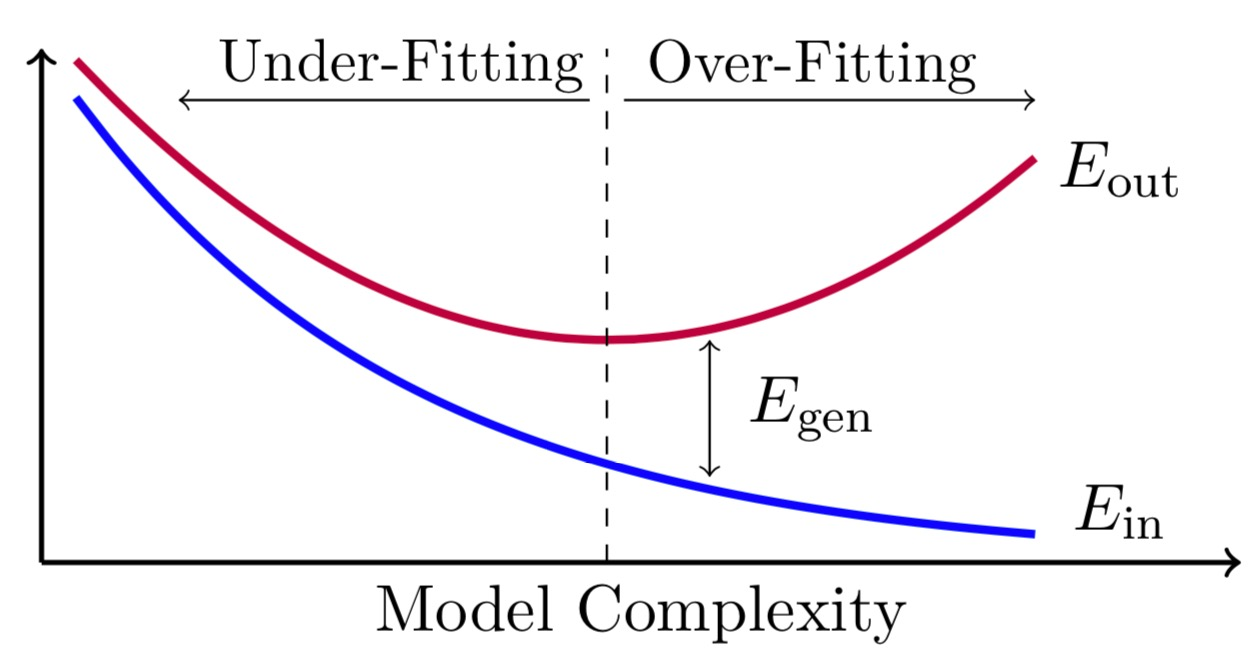
\includegraphics[width=.9\linewidth]{d_txtbook.jpg}
  \caption{\small figure from textbook}
  \label{fig:sub1}
\end{subfigure}%
\begin{subfigure}{.45\textwidth}
  \centering
  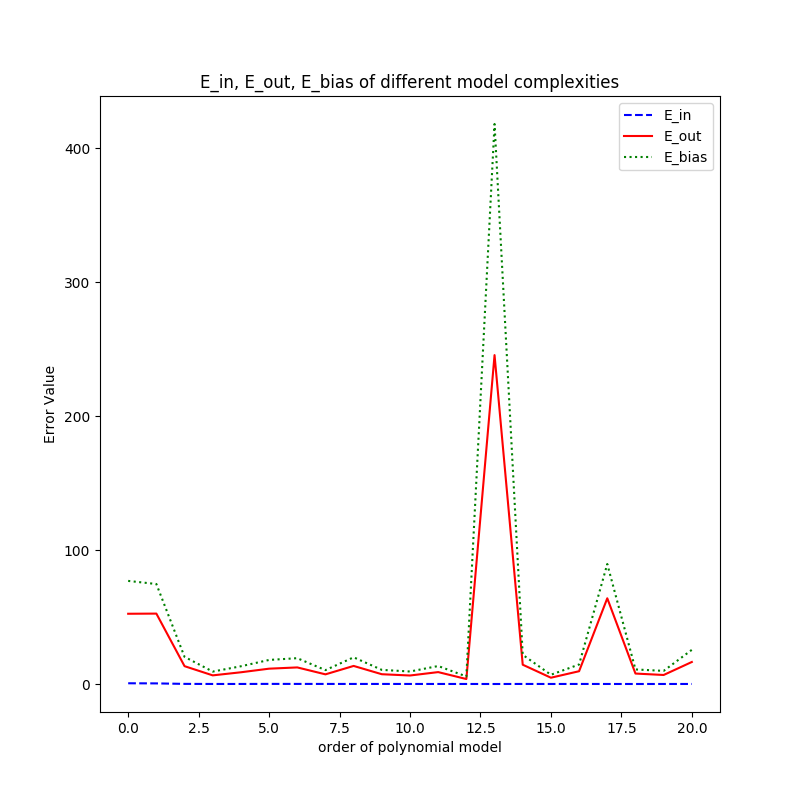
\includegraphics[width=.9\linewidth]{test_d_noreg.png}
  \caption{\small figure of test}
  \label{fig:sub2}
\end{subfigure}
\caption{\small Results of complexities.}
\label{fig:complex_nonreg}
\end{figure}

\subsubsection{Parameters Settings}
\begin{itemize}
    \item Complexity $d$: $d \in \{ 1, 2, ..., 20 \}$;
    \item Dataset size $N$: $N = 50$;
    \item Variance $\sigma$: $\sigma = 0.1$.
\end{itemize}

\subsubsection{Conclusion}

As the experiment shows, the result of the experiment basically followed what we learnt from the lecture. The out-of-sample error starts extremely high when the model is too simple to cover the dataset. A significant drop occurs after the complexity of the polynomial reaches around $3$ to $5$. The error gap ($E_{gap} = E_{out} - E_{in}$) reaches the minimal when the order becomes around $12 ~ 15$, and after that it goes up again. Thus, the over-fitting starts at order $12 ~ 15$ when the dataset size is $N = 50$.

The in-sample error $E_{in}$ shows a slightly decrease in the test figure. It is mainly because the variance is not that high and the number of training iteration is big, which makes the model learn well.

The bias error $E_{bias}$ follows almost the same trend as the result of $E_{out}$.

\subsection{Result of different sizes of dataset}

Then, dataset size is researched, the result is plotted as Figure~\ref{fig:size_nonreg} shows,
\begin{figure}[h]
\centering
\begin{subfigure}{.45\textwidth}
  \centering
  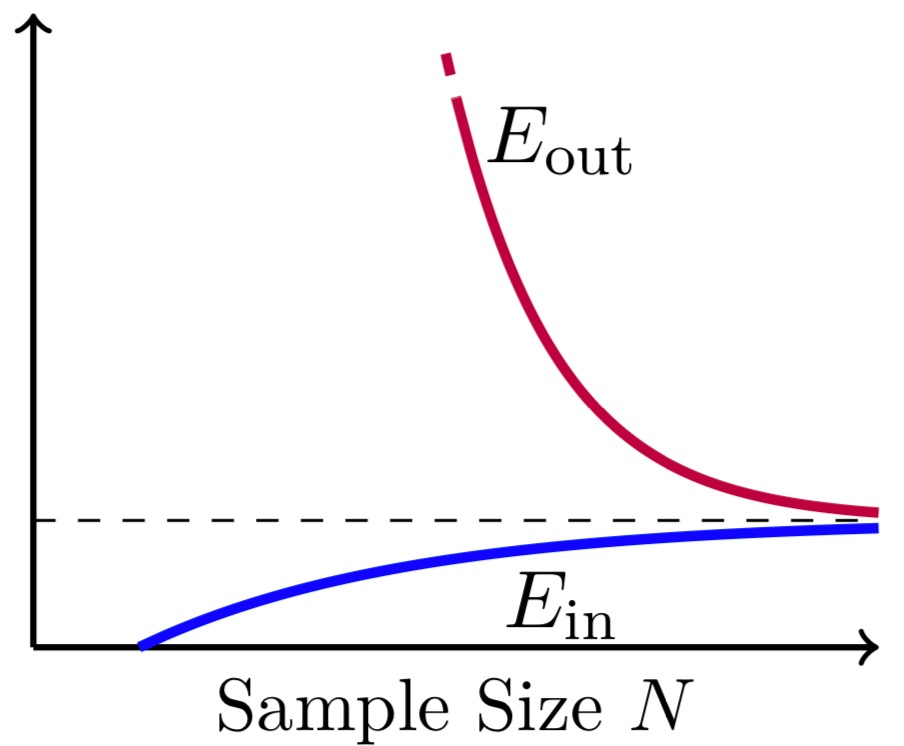
\includegraphics[width=.8\linewidth]{sample_txtbook.jpg}
  \caption{\small figure from textbook}
  \label{fig:sub1}
\end{subfigure}%
\begin{subfigure}{.45\textwidth}
  \centering
  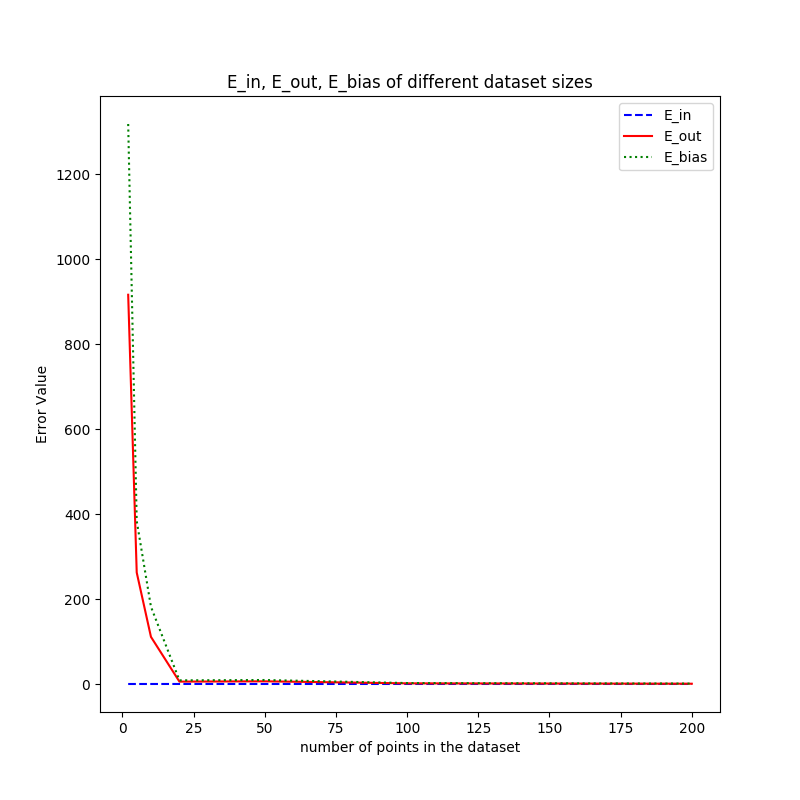
\includegraphics[width=.9\linewidth]{test_N_noreg.png}
  \caption{\small figure of test}
  \label{fig:sub2}
\end{subfigure}
\caption{\small Results of dataset size.}
\label{fig:size_nonreg}
\end{figure}

\subsubsection{Parameters Settings}
\begin{itemize}
    \item Complexity $d$: $d = 5$;
    \item Dataset size $N$: $N \in \{ 2,5,10,20,50,100,200 \}$;
    \item Variance $\sigma$: $\sigma = 0.1$.
\end{itemize}

\subsubsection{Conclusion}

As the experiment shows, the $E_{out}$ and $E_{bias}$ go all the way down and converge to a stable value just as the lecture slides indicate.

The $E_{in}$ increase slightly step-by-step, and finally reach the same level with $E_{out}$ and $E_{bias}$.

This implies that the larger the dataset, the smaller error gap we could get, and the better result the model could learn.

\subsection{Result of different dataset variance}

Then, dataset variance is researched, the result is plotted as Figure~\ref{fig:variance_nonreg} shows,
\begin{figure}[h]
\centering
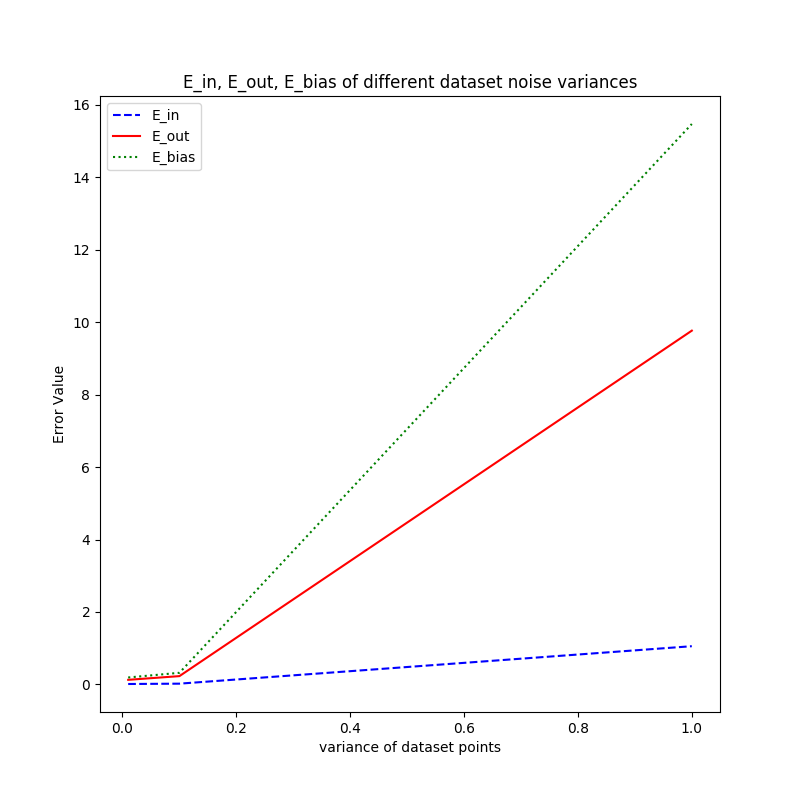
\includegraphics[width=.5\linewidth]{test_sigma_noreg.png}
\caption{\small Results of dataset variance.}
\label{fig:variance_nonreg}
\end{figure}

\subsubsection{Parameters Settings}
\begin{itemize}
    \item Complexity $d$: $d = 10$;
    \item Dataset size $N$: $N = 200$;
    \item Variance $\sigma$: $\sigma \in \{ 0.01, 0.1, 1 \}$.
\end{itemize}

\subsubsection{Conclusion}

As the experiment shows, all $E_{in}$, $E_{out}$ and $E_{bias}$ drametically increase during the whole changes with $E_{bias}$ and $E_{out}$ changing greater than $E_{in}$.

\section{Results with regularization}

Since we want to find the differences between regularized model and un-regularized model, in the following tests, only a new parameter is introduced with $\lambda_{reg} = 0.01$. All other parameters are kept the same. So, we will skip the \emph{paramters settings} part.

\subsection{Result of different model complexities}

The result comparison between complexity curve before regularization and after regularizaton is shown as Figure~\ref{fig:complex_reg},
\begin{figure}[h]
\centering
\begin{subfigure}{.45\textwidth}
  \centering
  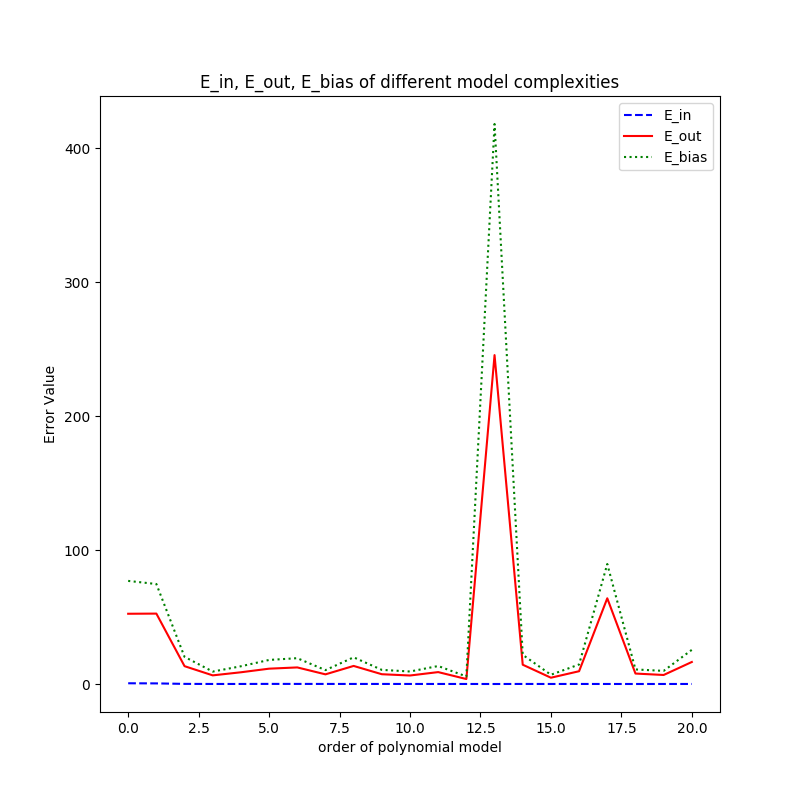
\includegraphics[width=.9\linewidth]{test_d_noreg.png}
  \caption{\small Un-regularized}
  \label{fig:sub1}
\end{subfigure}
\begin{subfigure}{.45\textwidth}
  \centering
  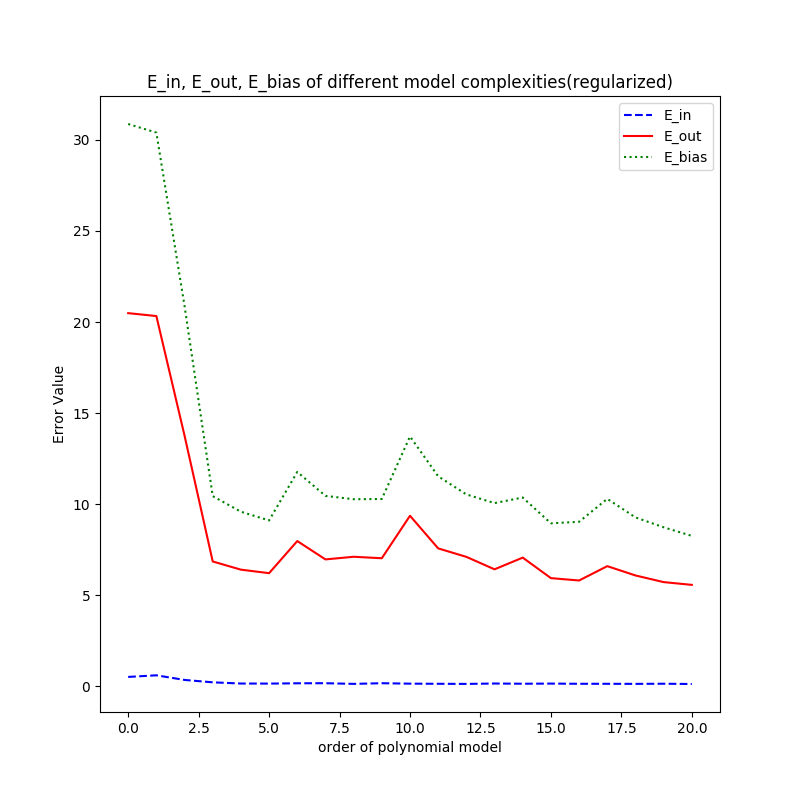
\includegraphics[width=.9\linewidth]{test_d_regularized.png}
  \caption{\small Regularized}
  \label{fig:sub2}
\end{subfigure}
\caption{\small Results of complexities.}
\label{fig:complex_reg}
\end{figure}

\subsubsection{Conclusion}

As the experiment shows, all $E_{in}$, $E_{out}$ and $E_{bias}$ drametically increase during the whole changes with $E_{bias}$ and $E_{out}$ changing greater than $E_{in}$.



% \end{lecture}

\end{document}
